\section*{\code{latex2plos} tests}

This section is not a part of the original PLOS \LaTeX~template.
It has been added to demonstrate the commonly used \LaTeX~features that are not present in the PLOS template, and verify that \code{latex2plos} is able to handle them properly.

\subsection*{\code{verbatiminput}}

\code{latex2plos.transformers.VerbatimInputTransformer} will transform a \verb|\verbatiminput| file inclusion into its equivalent \verb|\begin{verbatim}...\end{verbatim}| call, as in the example below \cite{Project:friendly_name_mixin:CodeRepository}:

\verbatiminput{listings/friendly_name_mixin.py}

\subsection*{\code{bibliography}}

\code{latex2plos.transformers.BibliographyTransformer} will transform a \verb|\bibliography| file inclusion into its equivalent \verb|\begin{thebibliography}...\end{thebibliography}| call, as demonstrated by this example paper (\code{paper.tex}) and its BiBTeX database (\code{references.bib}).

This is done as PLOS does not allow submission of BiBTeX databases, and instead requires the reference information to be embedded in the paper directly \cite{PLOS:LaTeX}.

\subsection*{\code{lstinputlisting}}

\code{latex2plos.transformers.InputListingTransformer} will copy over the files referenced by \verb|\lstinputlisting| into the papers export directory, as in the examples below:

\lstinputlisting[language=Python,caption={\code{friendly\_name\_mixin} project source code \cite{Project:friendly_name_mixin:CodeRepository}}]{listings/friendly_name_mixin.py}

\lstinputlisting[language=Python,caption={\code{friendly\_name\_mixin} project unit tests \cite{Project:friendly_name_mixin:CodeRepository}}]{listings/tests.py}

\subsection*{\code{includegraphics}}

\code{latex2plos.transformers.IncludeGraphicsTransformer} will copy over the figures referenced by \verb|\includegraphics| into the papers export directory, as shown in \cref{fig:petar-avatar,fig:3-clamped-free-beam-decimal-precision-errors,fig:barbero-viscoelastic-natural-frequencies,fig:barbero-viscoelastic-damage-analysis}.
It will also transform all figures into the TIFF image format (LZW compression, at 300 dpi) and remove/comment-out them from the papers exported PDF, as per PLOS requirements \cite{PLOS:LaTeX, PLOS:Figures}.

\begin{figure}[H]
    \centering
    
\includegraphics[height=6cm]{figures/petar-gravatar.png}
    \caption{Petar Marić gravatar (PNG image format) \cite{Maric:Gravatar}}
    \label{fig:petar-avatar}
\end{figure}

\begin{figure}[H]
    \centering
    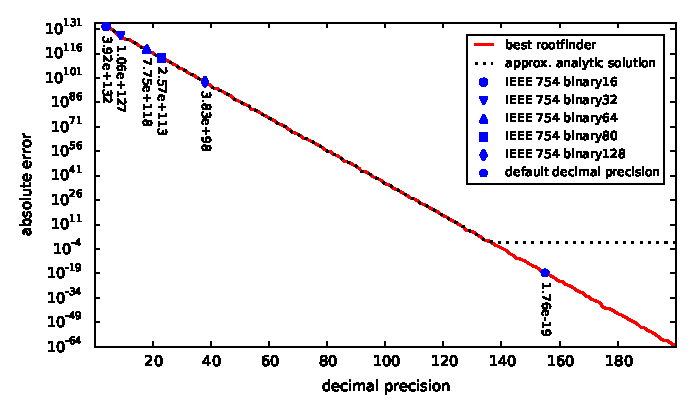
\includegraphics[width=\linewidth]{figures/decimal-precision-error@3-clamped-free-beam.eps}
    \caption{Maximum root-finding errors (across all 100 modes) of clamped-free beam's (LJ=3) characteristic function (EPS image format) \cite{Maric:2017}}
    \label{fig:3-clamped-free-beam-decimal-precision-errors}
\end{figure}

\begin{figure}[H]
    \centering
    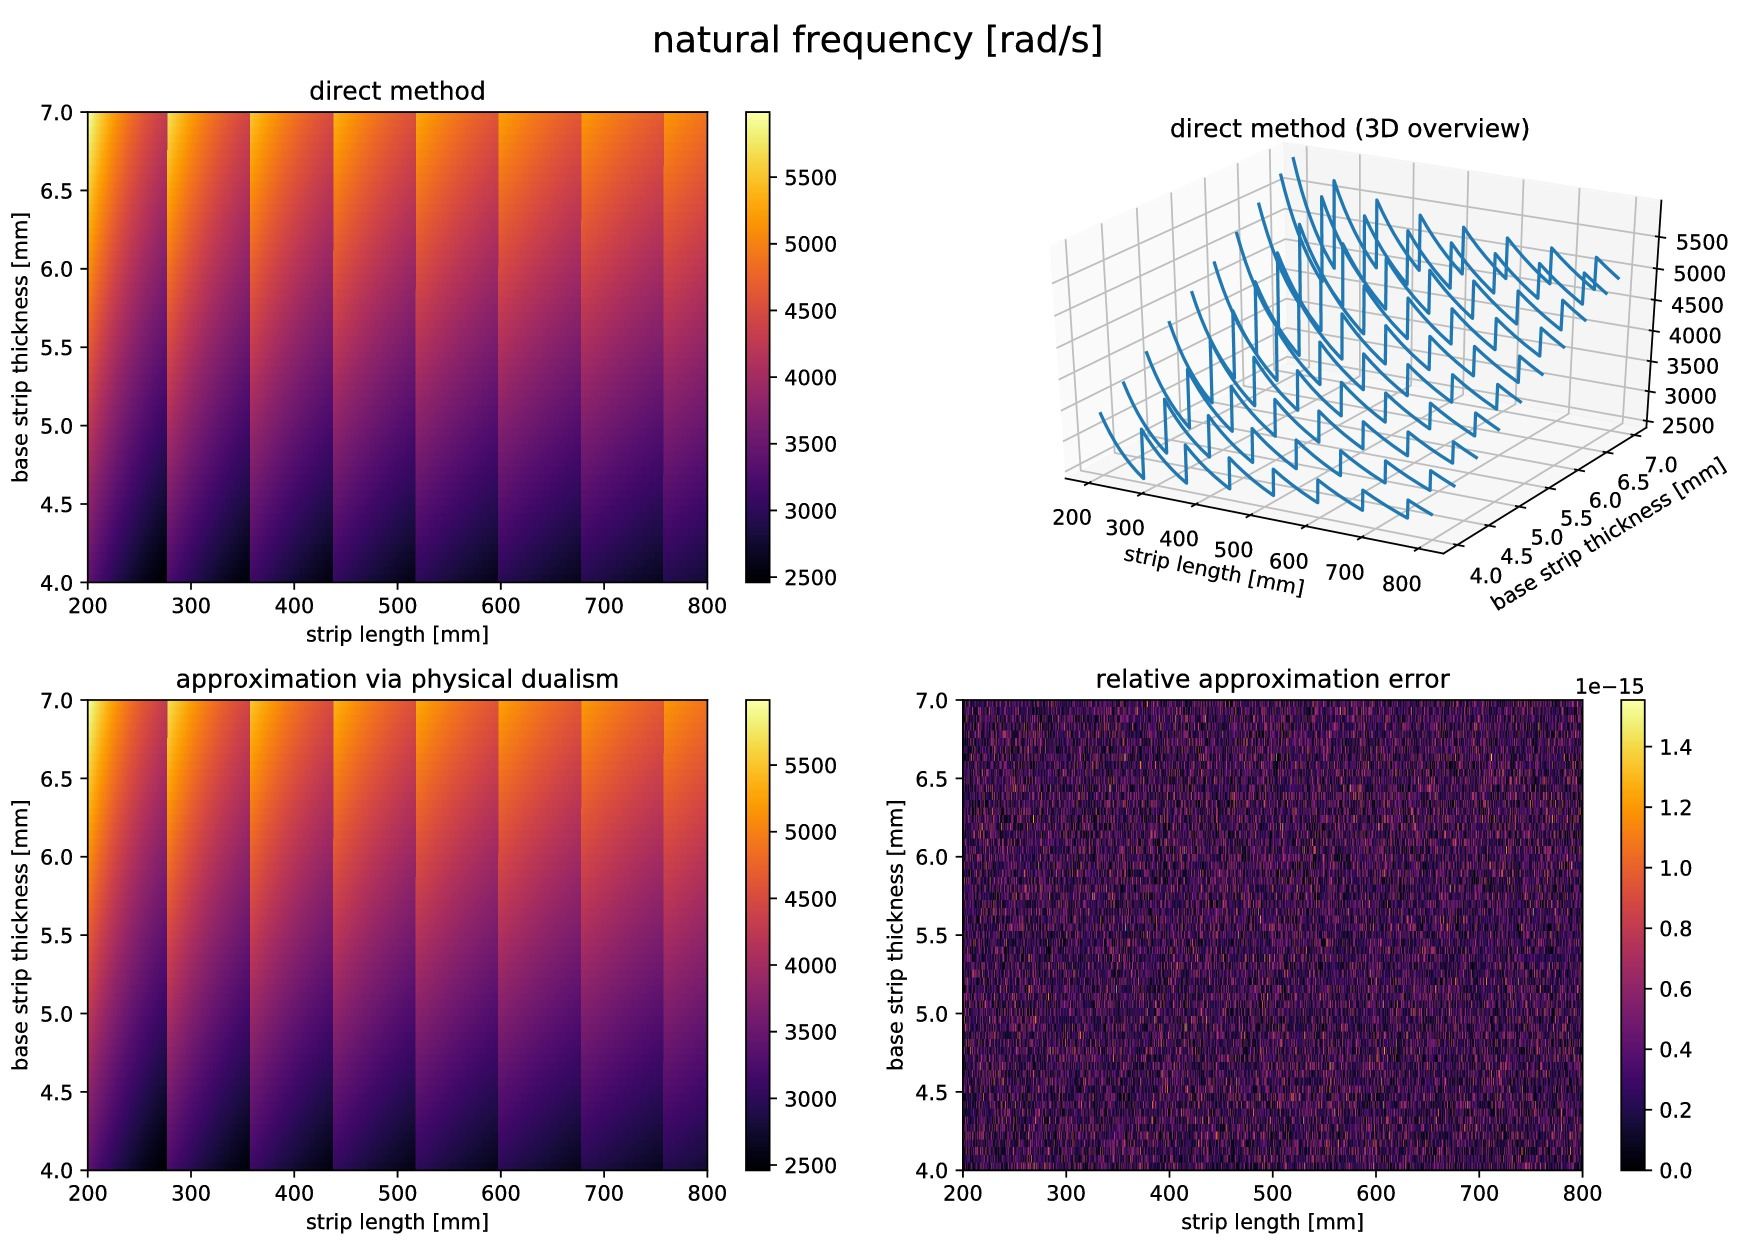
\includegraphics[width=\linewidth]{figures/barbero-viscoelastic@local-p1.jpg}
    \caption{Viscoelastic natural frequencies (JPEG image format) \cite{Milasinovic:2018}}
    \label{fig:barbero-viscoelastic-natural-frequencies}
\end{figure}

\begin{figure}[H]
    \centering
    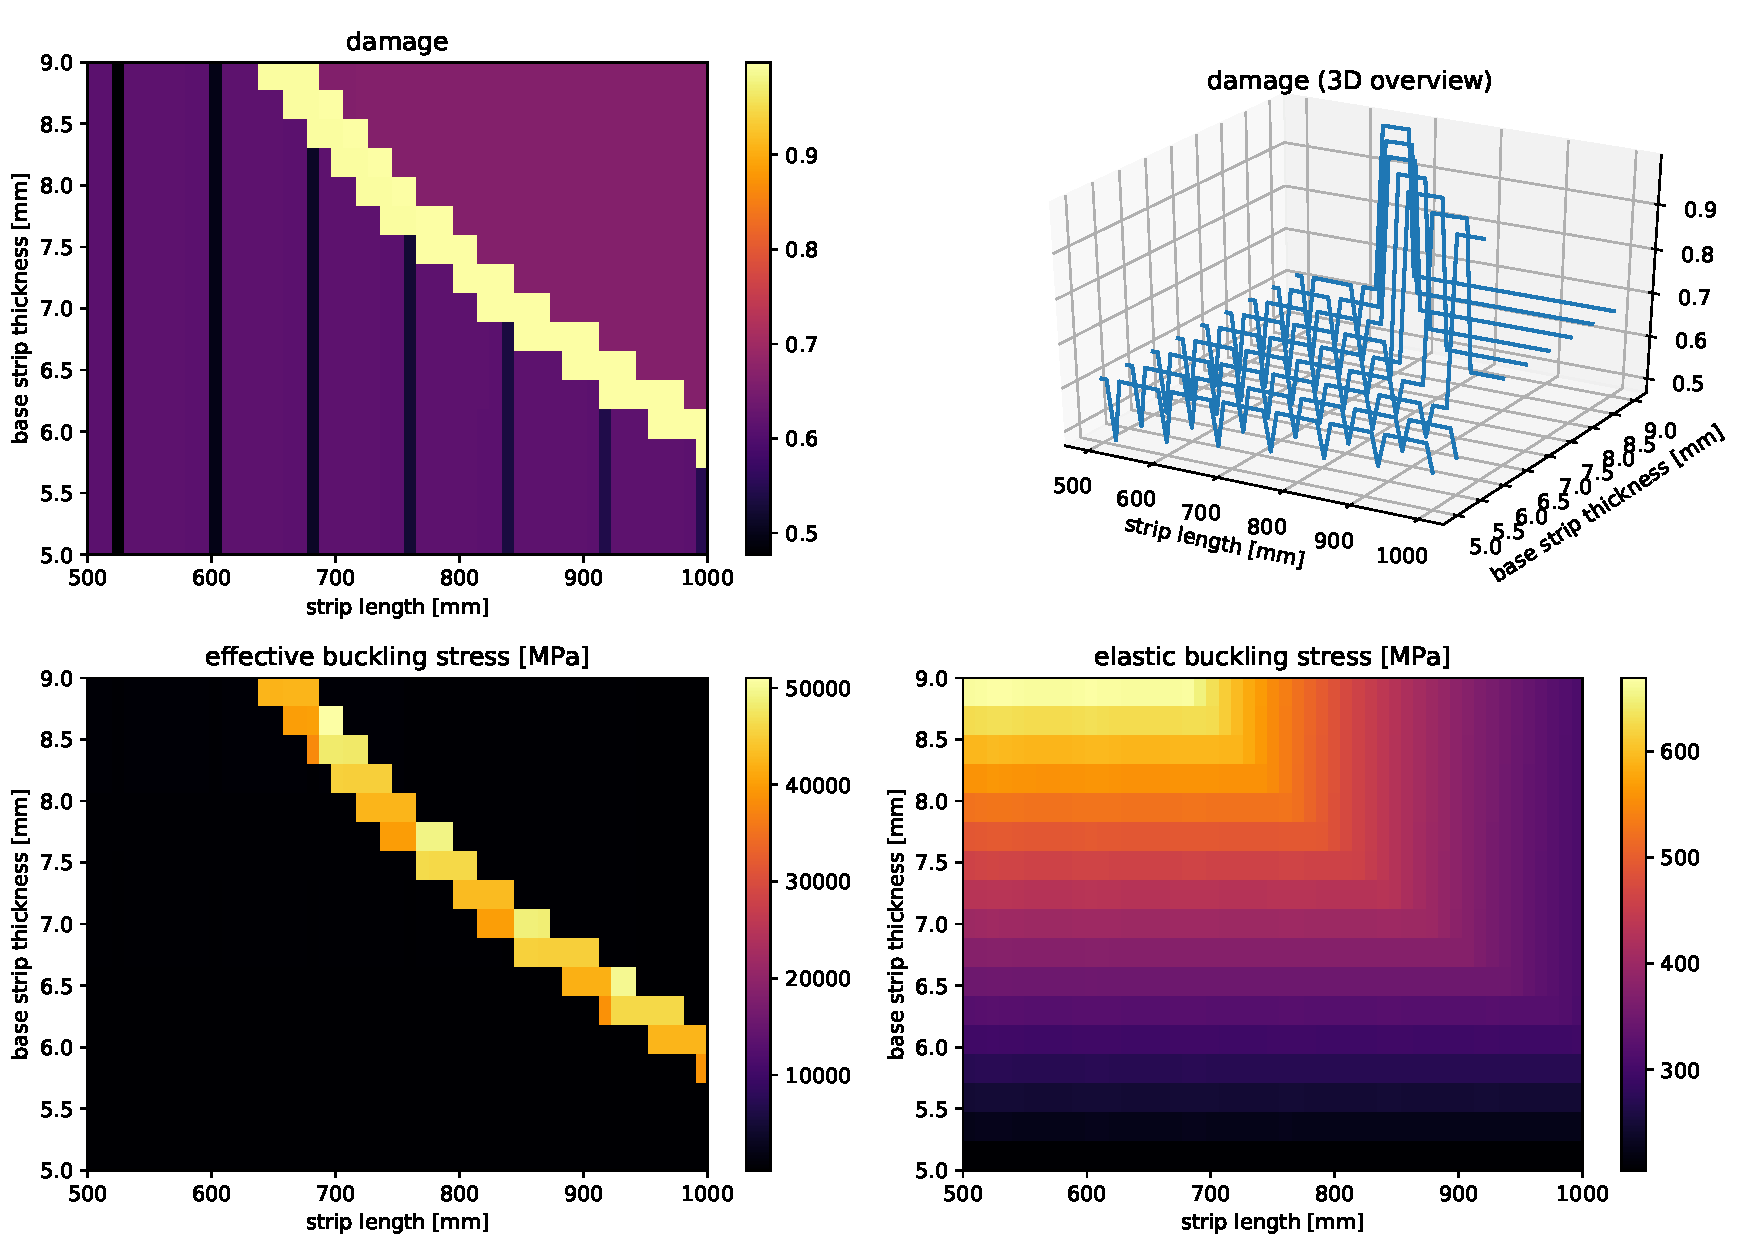
\includegraphics[width=\linewidth]{figures/barbero-viscoelastic@fsm-damage-analysis.pdf}
    \caption{\code{fsm\_damage\_analysis} project example experiment report (PDF image format) \cite{Project:fsm_damage_analysis:CodeRepository}}
    \label{fig:barbero-viscoelastic-damage-analysis}
\end{figure}

\subsection*{Multiple \LaTeX~files workflow}

\code{latex2plos.transformers.IncludeTransformer} will embed the contents of files referenced by \verb|\include| into the exported paper directly, whereas \code{latex2plos.transformers.InputTransformer} will do the same for \verb|\input|, as demonstrated by this example paper (\code{paper.tex}) and its referenced \code{.tex} files (\code{preamble.tex},  \code{head/*.tex} and \code{sections/*.tex}).

This is done as PLOS does not allow submission of multiple \code{.tex} files, and instead requires them to be combined into a single, cohesive \code{.tex} file \cite{PLOS:LaTeX}.
